\documentclass[a4paper, 12pt]{report}
\usepackage[utf8]{inputenc}
\usepackage[french]{babel}
\usepackage{amsmath}
\usepackage{listings}
\usepackage{xcolor}
\usepackage{hyperref}
\usepackage{graphicx}
\usepackage{float}
\usepackage[backend=biber,style=alphabetic,citestyle=authoryear]{biblatex}
\usepackage{fancyhdr}
\addbibresource{bibliographie.bib} % Nom du fichier .bib contenant les références



\title{Rapport : Introduction au langage d'assemblage}
\author{SANNA Thomas, L3STI}
\date{\today}

\pagestyle{fancy}
\fancyhead[L]{\leftmark} % Section courante à gauche
\fancyhead[R]{\thepage} % Numéro de page à droite
\fancyfoot[L]{Introduction au langage d'assemblage} % Titre du document à gauche
\fancyfoot[R]{SANNA Thomas, L3STI} % Nom de l'auteur à droite

\lstset{
  language=[x86masm]Assembler,
  basicstyle=\ttfamily\footnotesize,
  keywordstyle=\color{blue},
  commentstyle=\color{green!60!black},
  stringstyle=\color{red},
  numbers=left,
  numberstyle=\tiny\color{gray},
  stepnumber=1,
  numbersep=10pt,
  backgroundcolor=\color{lightgray!20},
  frame=single,
  rulecolor=\color{black},
  tabsize=4,
  captionpos=b,
  breaklines=true,
  breakatwhitespace=false,
  showspaces=false,
  showstringspaces=false,
  showtabs=false,
  morekeywords={section, global, mov, add, lea, int}
}

\begin{document}

\maketitle

\break

\newpage
\thispagestyle{empty}
\vspace*{\fill}
\begin{center}
  
\includegraphics[width=1\textwidth]{imgs/logouniv.jpg}
\end{center}
\vspace*{\fill}


\tableofcontents

\chapter{Introduction}
L'assembleur, ou langage d'assemblage, est un langage de programmation de bas niveau qui est étroitement lié à l'architecture matérielle d'un ordinateur. Contrairement aux langages de haut niveau comme le C ou le Python, l'assembleur permet de manipuler directement les registres et la mémoire de la machine.

\section{Qu'est-ce que l'assembleur?}
L'assembleur est un langage de programmation qui traduit les instructions du programmeur en code machine compréhensible par le processeur. Chaque instruction en assembleur correspond à une instruction machine spécifique, ce qui permet un contrôle très précis du matériel.

\section{Pourquoi utiliser l'assembleur?}
L'utilisation de l'assembleur présente plusieurs avantages:
\begin{itemize}
  \item \textbf{Performance}: Les programmes en assembleur peuvent être extrêmement rapides et efficaces car ils sont optimisés pour l'architecture spécifique du processeur.
  \item \textbf{Contrôle}: L'assembleur permet un contrôle total sur le matériel, ce qui est essentiel pour les systèmes embarqués, les pilotes de périphériques et les applications en temps réel.
  \item \textbf{Compréhension approfondie}: Apprendre l'assembleur aide à comprendre le fonctionnement interne des ordinateurs, ce qui peut être bénéfique pour le débogage et l'optimisation des programmes en langages de haut niveau.
\end{itemize}

\section{Inconvénients de l'assembleur}
Malgré ses avantages, l'assembleur présente également des inconvénients:
\begin{itemize}
  \item \textbf{Complexité}: La programmation en assembleur est complexe et nécessite une connaissance approfondie de l'architecture matérielle.
  \item \textbf{Portabilité}: Les programmes en assembleur sont spécifiques à une architecture de processeur particulière et ne peuvent pas être facilement portés sur d'autres architectures.
  \item \textbf{Temps de développement}: Écrire des programmes en assembleur prend généralement plus de temps que d'utiliser des langages de haut niveau en raison de la nécessité de gérer les détails de bas niveau.
\end{itemize}

\section{Comparaison entre un langage de haut niveau et l'assembleur}
Les langages de haut niveau, comme le Python, le C ou le Java, sont conçus pour être faciles à lire et à écrire pour les humains. Ils permettent aux développeurs de se concentrer sur la logique du programme sans se soucier des détails de l'architecture matérielle. Cependant, ces langages doivent être traduits en code machine compréhensible par le processeur, ce qui implique plusieurs étapes de compilation et d'interprétation.

\subsection{Langages de haut niveau}
Lorsqu'un programme est écrit dans un langage de haut niveau, il passe par plusieurs étapes avant d'être exécuté par le processeur:
\begin{enumerate}
  \item \textbf{Compilation}: Le code source est traduit en code intermédiaire (par exemple, bytecode pour Java) ou directement en code machine (comme pour le C).
  \item \textbf{Interprétation}: Pour certains langages comme Python, le code source est interprété ligne par ligne par un interpréteur, qui traduit chaque ligne en instructions machine à la volée.
  \item \textbf{Optimisation}: Les compilateurs modernes effectuent diverses optimisations pour améliorer les performances du code généré.
\end{enumerate}

\subsection{Langage assembleur}
En revanche, l'assembleur est beaucoup plus proche du matériel. Chaque instruction en assembleur correspond directement à une instruction machine spécifique. Voici les étapes typiques pour traduire un programme en assembleur en code machine:
\begin{enumerate}
  \item \textbf{Assemblage}: Le code assembleur est traduit en code machine par un assembleur.
  \item \textbf{Lien}: Les fichiers objets générés par l'assembleur sont liés pour créer un exécutable.
\end{enumerate}

\break\subsection{Comparaison}
\begin{itemize}
  \item \textbf{Abstraction}: Les langages de haut niveau offrent un niveau d'abstraction élevé, ce qui simplifie la programmation mais peut entraîner une perte de contrôle sur le matériel. L'assembleur, en revanche, offre un contrôle précis sur le matériel mais nécessite une connaissance approfondie de l'architecture du processeur.
  \item \textbf{Performance}: Les programmes en assembleur peuvent être extrêmement rapides et efficaces car ils sont optimisés pour l'architecture spécifique du processeur. Les langages de haut niveau dépendent des optimisations du compilateur pour atteindre des performances similaires.
  \item \textbf{Portabilité}: Les programmes en langages de haut niveau sont généralement plus portables entre différentes architectures matérielles. Les programmes en assembleur sont spécifiques à une architecture de processeur particulière.
  \item \textbf{Temps de développement}: Écrire des programmes en langages de haut niveau prend généralement moins de temps que d'utiliser l'assembleur en raison de la simplicité et de l'abstraction offertes par ces langages.
\end{itemize}

\begin{figure}[H]
  \centering
  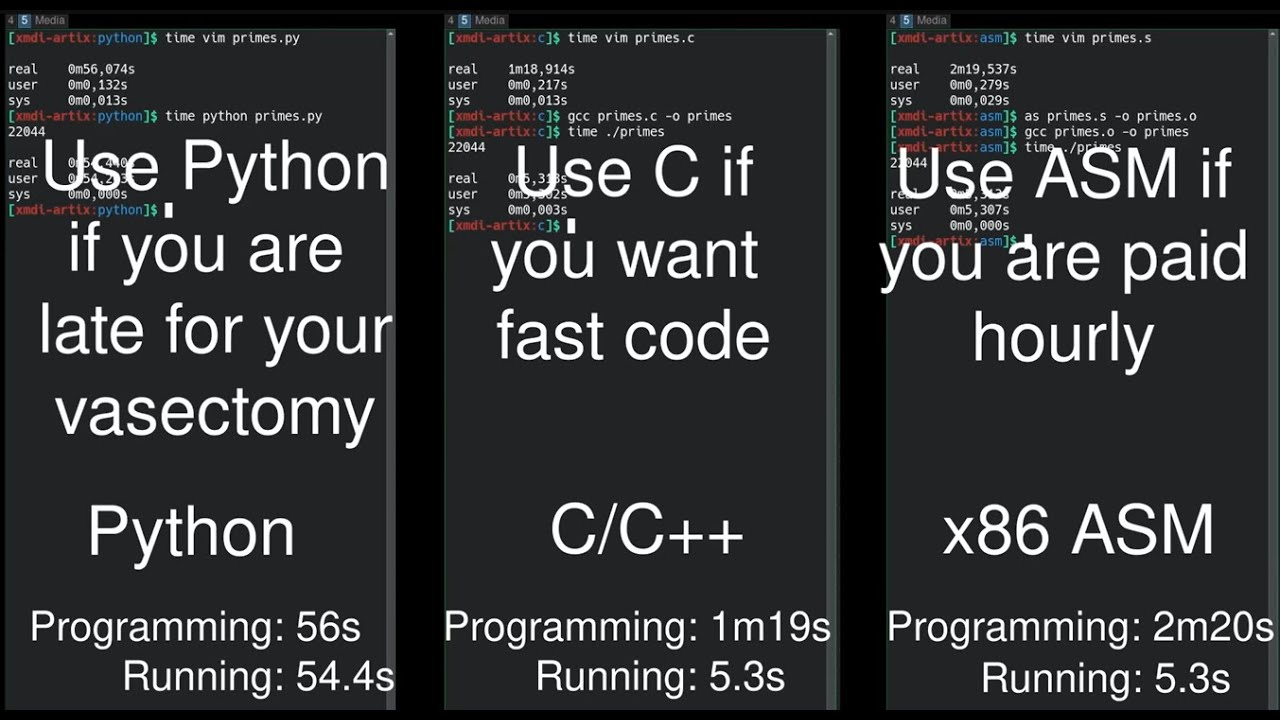
\includegraphics[width=0.8\textwidth]{imgs/compPythonAsm.jpg}
  \caption{Comparaison humoristique entre Python, C et ASM. Source : \url{https://www.youtube.com/watch?v=c-6SfKWmH0k} \cite{4}}
\end{figure}

\section{Applications de l'assembleur}
L'assembleur est utilisé dans plusieurs domaines spécifiques:
\begin{itemize}
  \item \textbf{Systèmes embarqués}: Les microcontrôleurs et autres systèmes embarqués utilisent souvent l'assembleur pour des performances optimales.
  \item \textbf{Développement de systèmes d'exploitation}: Les noyaux de systèmes d'exploitation et les pilotes de périphériques sont souvent écrits en assembleur pour un contrôle précis du matériel.
  \item \textbf{Optimisation de code}: Les sections critiques de certains programmes peuvent être écrites en assembleur pour maximiser les performances.
\end{itemize}

\chapter{Historique}
Le langage assembleur a été développé dans les années 1950 pour simplifier la programmation des premiers ordinateurs. Avant l'assembleur, les programmeurs devaient écrire des programmes en code machine, ce qui était extrêmement fastidieux et sujet aux erreurs.

\section{Les débuts de l'assembleur}
Les premiers ordinateurs, comme l'ENIAC et l'UNIVAC, utilisaient des commutateurs et des câbles pour programmer des instructions en code machine. Cela rendait la programmation très laborieuse et sujette aux erreurs. Pour simplifier ce processus, les langages assembleurs ont été créés. Le premier assembleur connu est celui développé pour l'EDSAC (Electronic Delay Storage Automatic Calculator) en 1949 par Maurice Wilkes et son équipe à l'Université de Cambridge.

\section{L'évolution des langages assembleurs}
Au fil des années, les langages assembleurs ont évolué pour s'adapter aux nouvelles architectures de processeurs. Chaque nouvelle génération de processeurs a introduit de nouvelles instructions et de nouvelles fonctionnalités, ce qui a conduit à la création de nouveaux assembleurs. Par exemple, l'assembleur pour le processeur IBM 704, développé dans les années 1950, a introduit des instructions pour les opérations en virgule flottante, ce qui a permis de réaliser des calculs plus complexes.

\section{L'assembleur et les mini-ordinateurs}
Dans les années 1960 et 1970, l'assembleur a joué un rôle crucial dans le développement des mini-ordinateurs. Les mini-ordinateurs, comme le PDP-8 de Digital Equipment Corporation (DEC), étaient plus petits et moins coûteux que les ordinateurs centraux, ce qui les rendait accessibles à un plus grand nombre d'utilisateurs. Les langages assembleurs pour ces machines ont permis aux programmeurs de tirer pleinement parti de leurs capacités limitées en optimisant les performances et l'utilisation de la mémoire.

\section{L'ère des microprocesseurs}
Avec l'avènement des microprocesseurs dans les années 1970, l'assembleur est devenu encore plus important. Les premiers microprocesseurs, comme l'Intel 4004 et le Motorola 6800, avaient des capacités limitées et nécessitaient une programmation en assembleur pour maximiser leur efficacité. L'assembleur a également été utilisé pour développer les premiers systèmes d'exploitation et logiciels pour micro-ordinateurs, comme le CP/M et le MS-DOS.

\section{L'assembleur aujourd'hui}
Aujourd'hui, l'assembleur est toujours utilisé dans des domaines spécifiques où la performance et le contrôle du matériel sont essentiels. Les systèmes embarqués, les pilotes de périphériques, les noyaux de systèmes d'exploitation et les applications en temps réel sont souvent développés en assembleur. De plus, l'assembleur est utilisé pour optimiser les sections critiques de certains programmes écrits en langages de haut niveau.

\section{L'impact de l'assembleur sur l'informatique}
L'assembleur a eu un impact profond sur le développement de l'informatique. Il a permis de simplifier la programmation des premiers ordinateurs, de tirer pleinement parti des capacités des mini-ordinateurs et des microprocesseurs, et de développer des logiciels performants et efficaces. Apprendre l'assembleur aide également à comprendre le fonctionnement interne des ordinateurs, ce qui est bénéfique pour le débogage et l'optimisation des programmes en langages de haut niveau.

\chapter{Architecture matérielle}
Pour comprendre l'assembleur, il est essentiel de connaître les composants de base d'un ordinateur:

\section{Unité centrale de traitement (CPU)}
L'unité centrale de traitement, ou CPU (Central Processing Unit), est le cerveau de l'ordinateur. Elle exécute les instructions des programmes en effectuant des opérations arithmétiques, logiques, de contrôle et d'entrée/sortie. Le CPU est composé de plusieurs sous-composants clés:
\begin{itemize}
  \item \textbf{Unité arithmétique et logique (ALU)}: Effectue les opérations arithmétiques et logiques.
  \item \textbf{Unité de contrôle}: Dirige les opérations du CPU en récupérant les instructions de la mémoire, en les décodant et en les exécutant.
  \item \textbf{Registres}: Petites unités de stockage à accès rapide utilisées pour stocker temporairement des données et des instructions.
  \item \textbf{Cache}: Mémoire rapide située à l'intérieur du CPU pour stocker les données fréquemment utilisées et réduire les temps d'accès.
\end{itemize}

\begin{figure}[H]
  \centering
  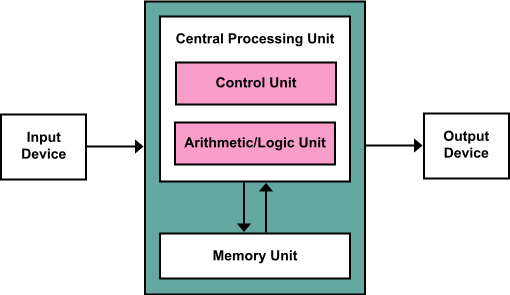
\includegraphics[width=0.8\textwidth]{imgs/Cpu_diagram.jpg}
  \caption{Architecture de base d'un CPU. Source : \url{https://computersciencewiki.org/index.php?title=File:Cpu_diagram.png} (\cite{5})}
\end{figure}

\section{Mémoire (RAM)}
La mémoire vive, ou RAM (Random Access Memory), est utilisée pour stocker les données et les instructions pendant leur utilisation. La RAM est volatile, ce qui signifie qu'elle perd son contenu lorsque l'ordinateur est éteint. Elle est organisée en cellules de mémoire, chacune ayant une adresse unique.

\section{Bus}
Les bus sont des systèmes de communication qui transfèrent les données entre les composants de l'ordinateur. Il existe plusieurs types de bus:
\begin{itemize}
  \item \textbf{Bus de données}: Transporte les données entre le CPU, la mémoire et les périphériques.
  \item \textbf{Bus d'adresse}: Transporte les adresses de mémoire des données que le CPU doit lire ou écrire.
  \item \textbf{Bus de contrôle}: Transporte les signaux de contrôle et de commande entre le CPU et les autres composants.
\end{itemize}

\section{Mémoire cache}
La mémoire cache est une mémoire rapide située à l'intérieur du CPU ou à proximité. Elle stocke les données fréquemment utilisées pour réduire les temps d'accès et améliorer les performances. Il existe généralement plusieurs niveaux de cache (L1, L2, L3), chaque niveau étant plus rapide mais plus petit que le précédent.

\section{Périphériques d'entrée/sortie (I/O)}
Les périphériques d'entrée/sortie permettent à l'ordinateur de communiquer avec le monde extérieur. Ils incluent des dispositifs tels que les claviers, les souris, les écrans, les imprimantes et les disques durs. Les opérations d'entrée/sortie sont souvent gérées par des contrôleurs spécifiques et peuvent être programmées en assembleur pour un contrôle précis.

\section{Architecture de Harvard vs. Architecture de von Neumann}
Il existe deux principales architectures de systèmes informatiques:
\begin{itemize}
  \item \textbf{Architecture de von Neumann}: Utilise un seul bus pour les instructions et les données, ce qui peut entraîner des goulots d'étranglement.
  \item \textbf{Architecture de Harvard}: Utilise des bus séparés pour les instructions et les données, permettant des accès simultanés et améliorant les performances.
\end{itemize}

\begin{figure}[H]
  \centering
  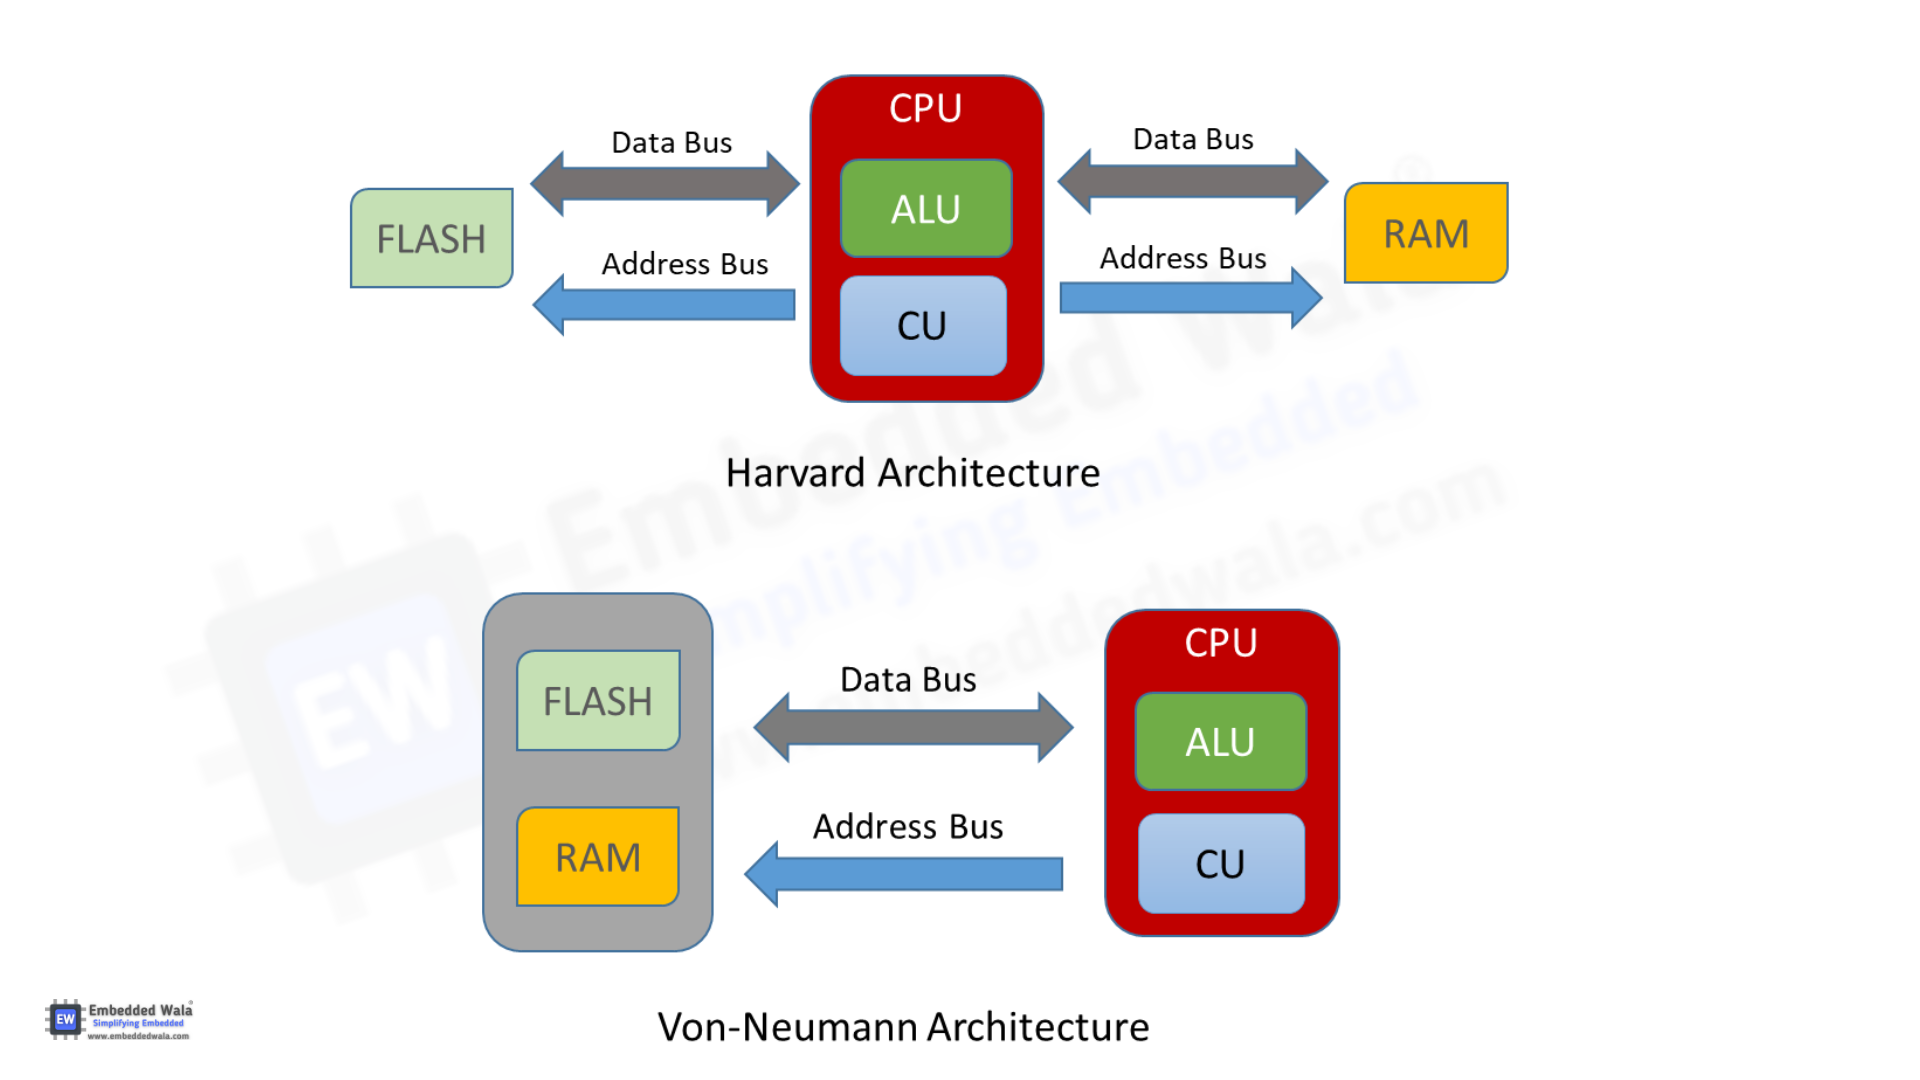
\includegraphics[width=0.8\textwidth]{imgs/neumann.jpg}
  \caption{Architecture de von Neumann vs. Architecture de Harvard. Source : \url{https://embeddedwala.com/Blogs/embeddedsystem/harvard-vs-von-neumann-architecture} (\cite{6})}
\end{figure}

\chapter{Notions de base en assembleur}

\section{Définition de variables}
En assembleur, les variables sont des emplacements de mémoire utilisés pour stocker des données. Les variables peuvent être déclarées dans différentes sections du programme, telles que la section .data ou la section .bss. Voici comment déclarer des variables en assembleur:

\subsection{Déclaration de variables dans la section .data}
Les variables déclarées dans la section .data sont initialisées avec des valeurs spécifiques. Voici un exemple de déclaration de variables dans la section .data:

\begin{lstlisting}[language={[x86masm]Assembler}]
  section .data
    message db "Hello, World!", 10  ; Declare une chaine de caracteres avec un saut de ligne a la fin (10 en ASCII)
    number db 42  ; Declare un octet (db = define byte) (8 bits)
    mot dw 1234  ; Declare un mot (dw = define word) (16 bits)
    dmot dd 12345678  ; Declare un double mot (dd = define double) (32 bits)
    qmot dq 1234567890123456789  ; Declare un quadruple mot (dq = define quadruple) (64 bits)
\end{lstlisting}

\subsection{Déclaration de variables dans la section .bss}
Les variables déclarées dans la section .bss ne sont pas initialisées avec des valeurs spécifiques.

\section{Instructions}
Les instructions en assembleur sont des commandes simples qui disent au CPU quoi faire. Chaque instruction correspond généralement à une opération de bas niveau, comme déplacer des données ou effectuer une opération arithmétique. Voici quelques-unes des instructions de base les plus couramment utilisées en assembleur \cite{2}:

\subsection{MOV}
L'instruction `mov` est utilisée pour copier des données d'un emplacement à un autre. Elle peut copier des données entre des registres, de la mémoire vers un registre, d'un registre vers la mémoire, ou charger une valeur immédiate dans un registre.

\begin{lstlisting}[language={[x86masm]Assembler}]
mov eax, ebx    ; Copier la valeur de ebx dans eax
mov eax, [var]  ; Charger la valeur de la variable var dans eax
mov [var], eax  ; Stocker la valeur de eax dans la variable var
mov eax, 10     ; Charger la valeur immzdiate 10 dans eax
\end{lstlisting}

\break\subsection{ADD}
L'instruction `add` est utilisée pour additionner deux opérandes. Le résultat est stocké dans le premier opérande.

\begin{lstlisting}[language={[x86masm]Assembler}]
add eax, ebx    ; Ajouter la valeur de ebx a eax
add eax, [var]  ; Ajouter la valeur de la variable var a eax
add [var], eax  ; Ajouter la valeur de eax a la variable var
add eax, 10     ; Ajouter la valeur immediate 10 a eax
\end{lstlisting}

\subsection{CMP}
L'instruction `cmp` est utilisée pour comparer deux opérandes. Elle soustrait le second opérande du premier et met à jour les drapeaux du registre FLAGS sans stocker le résultat.

\begin{lstlisting}[language={[x86masm]Assembler}]
cmp eax, ebx    ; Comparer eax et ebx
cmp eax, [var]  ; Comparer eax et la valeur de la variable var
cmp eax, 10     ; Comparer eax et la valeur immediate 10
\end{lstlisting}

Il existe encore beaucoup d'autres instructions en assembleur, mais celles-ci sont les plus couramment utilisées.

\section{Registres}

\begin{figure}[H]
  \centering
  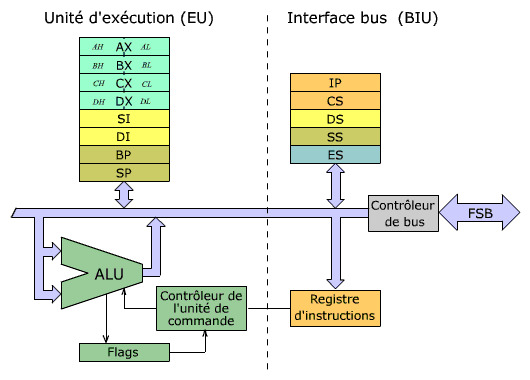
\includegraphics[width=0.8\textwidth]{imgs/registres.jpg}
  \caption{Registres du processeur x86. Source : (\cite{1})}
\end{figure}

Les registres sont des emplacements de stockage internes au CPU. Ils sont utilisés pour stocker temporairement des données pendant l'exécution des instructions. Les registres couramment utilisés incluent:

\subsection{Registres généraux}
Les registres généraux sont utilisés pour diverses opérations arithmétiques, logiques et de manipulation de données. Les registres généraux incluent AX, BX, CX et DX, chacun ayant des sous-parties spécifiques.

\begin{itemize}
  \item \textbf{AX (Accumulator Register)}: Utilisé principalement pour les \\opérations arithmétiques et logiques. Il est souvent impliqué dans les opérations de multiplication et de division. AX peut être divisé en deux registres de 8 bits: AH (High byte) et AL (Low byte).
    \begin{itemize}
      \item \textbf{AH}: Partie haute du registre AX. 
      \item \textbf{AL}: Partie basse du registre AX.
    \end{itemize}
    NB: Il y a une partie haute et une partie basse pour chaque registre général.
  \item \textbf{BX (Base Register)}: Utilisé comme pointeur de base pour accéder aux données en mémoire. Il est souvent utilisé dans les opérations de calcul d'adresse. BX peut également être divisé en BH (High byte) et BL (Low byte).
  \item \textbf{CX (Count Register)}: Utilisé principalement comme compteur dans les boucles et les opérations de chaîne. Par exemple, il est utilisé par les instructions de répétition comme `LOOP`, `REP`, `REPE`, et `REPNE`. CX peut être divisé en CH (High byte) et CL (Low byte).
  \item \textbf{DX (Data Register)}: Utilisé pour les opérations d'entrée/sortie et certaines opérations arithmétiques. Par exemple, il est utilisé en combinaison avec AX pour les opérations de multiplication et de division de grande taille. DX peut être divisé en DH (High byte) et DL (Low byte).
\end{itemize}

\subsection{Registres de segment}
Les registres de segment sont utilisés pour accéder à différentes sections de la mémoire. Ils incluent CS, DS, SS et ES.
\begin{itemize}
  \item \textbf{CS (Code Segment)}: Contient l'adresse de base du segment de code, où les instructions du programme sont stockées.
  \item \textbf{DS (Data Segment)}: Contient l'adresse de base du segment de données, où les variables sont stockées.
  \item \textbf{SS (Stack Segment)}: Contient l'adresse de base du segment de pile, utilisé pour la gestion de la pile d'exécution.
  \item \textbf{ES (Extra Segment)}: Utilisé comme segment supplémentaire pour les opérations de chaîne et autres opérations de données.
\end{itemize}

\subsection{Registres de pointeur et d'index}
Les registres de pointeur et d'index sont utilisés pour le calcul d'adresse et la manipulation de données.
\begin{itemize}
  \item \textbf{SP (Stack Pointer)}: Pointeur de pile, utilisé pour gérer la pile d'exécution. Il pointe vers le sommet de la pile.
  \item \textbf{BP (Base Pointer)}: Pointeur de base, utilisé pour accéder aux variables locales dans la pile. Il est souvent utilisé pour les appels de fonctions.
  \item \textbf{SI (Source Index)}: Utilisé pour les opérations de chaîne et les transferts de données. Il pointe vers la source des données.
  \item \textbf{DI (Destination Index)}: Utilisé pour les opérations de chaîne et les transferts de données. Il pointe vers la destination des données.
\end{itemize}

\subsection{Registre d'instruction et de drapeaux}
\begin{itemize}
  \item \textbf{IP (Instruction Pointer)}: Pointeur d'instruction, contient l'adresse de la prochaine instruction à exécuter.
  \item \textbf{FLAGS (Registre de drapeaux)}: Contient des indicateurs de statut qui reflètent les résultats des opérations. Les drapeaux incluent le drapeau de zéro (ZF), le drapeau de transport (CF), le drapeau de signe (SF), et d'autres.
\end{itemize}

\section{Pointeurs}
Les pointeurs sont des variables qui contiennent des adresses mémoire. En assembleur, les pointeurs sont souvent utilisés pour accéder directement à la mémoire. Comprendre les pointeurs est crucial pour manipuler efficacement les données en assembleur.

\subsection{Concept de pointeur}
Un pointeur est une variable qui stocke l'adresse mémoire d'une autre variable. Par exemple, si une variable \texttt{A} est stockée à l'adresse mémoire \texttt{0x1000}, un pointeur \texttt{P} peut contenir la valeur \texttt{0x1000}. Cela permet au programme d'accéder directement à la valeur de \texttt{A} en utilisant \texttt{P}.

\subsection{Utilisation des pointeurs en assembleur}
En assembleur, les pointeurs sont utilisés pour manipuler les données en mémoire de manière efficace. Voici quelques exemples d'utilisation des pointeurs en assembleur:

\begin{itemize}
  \item \textbf{Accès direct à la mémoire}: Les pointeurs permettent d'accéder directement aux adresses mémoire, ce qui est essentiel pour les opérations de bas niveau.
  \item \textbf{Manipulation de tableaux}: Les pointeurs sont utilisés pour parcourir et manipuler les éléments des tableaux.
  \item \textbf{Gestion de la pile}: Les pointeurs sont utilisés pour gérer la pile d'exécution, en particulier pour les appels de fonctions et la gestion des variables locales.
\end{itemize}



\chapter{Installation et exécution de l'assembleur}
Maintenant que l'on a appris tout cela, il est nécessaire d'installer un assembleur pour pouvoir écrire et exécuter des programmes en assembleur. Voici comment installer un assembleur sur Windows, Linux et macOS.

\section{Installation sur Windows}
Pour installer un assembleur sur Windows, nous utiliserons NASM (Netwide Assembler), un assembleur populaire pour le langage assembleur x86.

\subsection{Étapes d'installation}
\begin{enumerate}
  \item Téléchargez NASM depuis le site officiel: \url{https://www.nasm.us/}
  \item Exécutez le fichier d'installation et suivez les instructions pour installer NASM.
  \item Ajoutez le répertoire d'installation de NASM à la variable d'environnement PATH pour pouvoir l'exécuter depuis n'importe quel répertoire dans l'invite de commandes.
\end{enumerate}

\subsection{Compilation et exécution d'un programme en assembleur}
\begin{enumerate}
  \item Ouvrez un éditeur de texte (comme Notepad++) et écrivez votre programme en assembleur. Enregistrez le fichier avec l'extension `.asm`.
  \item Ouvrez l'invite de commandes et naviguez jusqu'au répertoire contenant votre fichier `.asm`.
  \item Compilez le programme en utilisant la commande suivante:
  \begin{lstlisting}[language=bash]
  nasm -f win32 programme.asm -o programme.obj
  \end{lstlisting}
  \item Liez le fichier objet pour créer un exécutable:
  \begin{lstlisting}[language=bash]
  gcc programme.obj -o programme.exe
  \end{lstlisting}
  \item Exécutez le programme:
  \begin{lstlisting}[language=bash]
  programme.exe
  \end{lstlisting}
\end{enumerate}

\section{Installation sur Linux}
Sur Linux, NASM est également disponible et peut être installé via le gestionnaire de paquets.

\subsection{Étapes d'installation}
\begin{enumerate}
  \item Ouvrez un terminal.
  \item Installez NASM en utilisant le gestionnaire de paquets de votre distribution. Par exemple, sur Debian/Ubuntu, utilisez la commande suivante:
  \begin{lstlisting}[language=bash]
  sudo apt-get install nasm
  \end{lstlisting}
\end{enumerate}

\subsection{Compilation et exécution d'un programme en assembleur}
\begin{enumerate}
  \item Ouvrez un éditeur de texte (comme gedit ou vim) et écrivez votre programme en assembleur. Enregistrez le fichier avec l'extension `.asm`.
  \item Ouvrez un terminal et naviguez jusqu'au répertoire contenant votre fichier `.asm`.
  \item Compilez le programme en utilisant la commande suivante:
  \begin{lstlisting}[language=bash]
  nasm -f elf32 programme.asm -o programme.o
  \end{lstlisting}
  \item Liez le fichier objet pour créer un exécutable:
  \begin{lstlisting}[language=bash]
  ld -m elf_i386 -s -o programme programme.o
  \end{lstlisting}
  \item Exécutez le programme:
  \begin{lstlisting}[language=bash]
  ./programme
  \end{lstlisting}
\end{enumerate}

\section{Installation sur macOS}
Sur macOS, vous pouvez également utiliser NASM.

\subsection{Étapes d'installation}
\begin{enumerate}
  \item Installez Homebrew si ce n'est pas déjà fait en suivant les instructions sur \url{https://brew.sh/}.
  \item Installez NASM en utilisant Homebrew:
  \begin{lstlisting}[language=bash]
  brew install nasm
  \end{lstlisting}
\end{enumerate}

\subsection{Compilation et exécution d'un programme en assembleur}
\begin{enumerate}
  \item Ouvrez un éditeur de texte (comme TextEdit ou vim) et écrivez votre programme en assembleur. Enregistrez le fichier avec l'extension `.asm`.
  \item Ouvrez un terminal et naviguez jusqu'au répertoire contenant votre fichier `.asm`.
  \item Compilez le programme en utilisant la commande suivante:
  \begin{lstlisting}[language=bash]
  nasm -f macho32 programme.asm -o programme.o
  \end{lstlisting}
  \item Liez le fichier objet pour créer un exécutable:
  \begin{lstlisting}[language=bash]
  ld -macosx_version_min 10.7.0 -o programme programme.o -lSystem
  \end{lstlisting}
  \item Exécutez le programme:
  \begin{lstlisting}[language=bash]
  ./programme
  \end{lstlisting}
\end{enumerate}



\chapter{Exemples de programme en assembleur}
Avant de montrer un exemple de programme en assembleur, il est important de comprendre comment est composé un code assembleur. Un programme en assembleur est généralement divisé en plusieurs sections, chacune ayant un rôle spécifique.

\section{Composition d'un code assembleur}
Un programme en assembleur est typiquement composé des sections suivantes :

\begin{itemize}
  \item \textbf{Section .data} : Cette section est utilisée pour déclarer les données statiques ou globales. Les variables définies ici sont accessibles tout au long de l'exécution du programme.
  \item \textbf{Section .bss} : Cette section est utilisée pour déclarer les variables non initialisées. Elle est similaire à la section .data, mais les variables ne sont pas initialisées avec des valeurs spécifiques.
  \item \textbf{Section .text} : Cette section contient le code exécutable du programme. C'est ici que les instructions du programme sont écrites.
\end{itemize}

\subsection{Commentaires}
Les commentaires en assembleur sont utilisés pour expliquer le code et sont ignorés par l'assembleur. Ils commencent par un point-virgule (`;`).

\subsection{Directives (ou Sections)}
Les directives sont des instructions spéciales pour l'assembleur. Elles commencent généralement par un point (`.`) et ne sont pas traduites en instructions machine. Par exemple, `.data`, `.bss`, et `.text` sont des directives.

\section{Exemple de programme en assembleur : Addition de deux nombres}
Voici un exemple simple de programme en assembleur qui additionne deux nombres :

\begin{lstlisting}[language={[x86masm]Assembler}]
section .data
  num1 db 5       ; Declaration de la variable num1 avec la valeur 5. (db = define byte)
  num2 db 10      ; Declaration de la variable num2 avec la valeur 10
  result db 0     ; Declaration de la variable result initialisee a 0

section .text
  global _start   ; Declaration de l'etiquette globale _start

_start:
  mov al, [num1]  ; Charger la valeur de num1 dans le registre AL
  add al, [num2]  ; Ajouter la valeur de num2 a AL
  mov [result], al ; Stocker le resultat dans result

  ; Exit
  mov rax, 60      ; Code de sortie pour l'appel systeme
  xor rdi, rdi     ; Code de retour (0 signifie succes)
  syscall          ; Appel systeme pour terminer le programme
\end{lstlisting}

\break\section{Exemple de programme en assembleur : Lecture de données}
Voici un exemple de programme en assembleur qui lit une chaîne de caractères depuis l'entrée standard et l'affiche :

\begin{lstlisting}[language={[x86masm]Assembler}]
section .bss ; "bss" sert a declarer des variables non initialisees
  buffer resb 128  ; Reserver 128 octets pour le buffer.

section .data
  msg db "Entrez une chaine de caracteres: ", 0

section .text
  global _start

_start:
    ; Afficher le message
    mov rax, 1          ; Code de l'appel systeme pour 'write' (1)
    mov rdi, 1          ; Descripteur de fichier pour stdout (1)
    mov rsi, msg        ; Adresse du message a afficher
    mov rdx, 35         ; Longueur du message
    syscall             ; Effectuer l'appel systeme 'write(1, msg, 35)'

    ; Lire l'entree du clavier
    mov rax, 0          ; Code de l'appel systeme pour 'read' (0)
    mov rdi, 0          ; Descripteur de fichier pour stdin (0)
    mov rsi, buffer     ; Adresse du buffer ou stocker l'entree
    mov rdx, 128        ; Taille maximale de l'entree
    syscall             ; Effectuer l'appel systeme 'read(0, buffer, 128)'

    ; Afficher l'entree lue
    mov rax, 1          ; Code de l'appel systeme pour 'write' (1)
    mov rdi, 1          ; Descripteur de fichier pour stdout (1)
    mov rsi, buffer     ; Adresse du buffer contenant l'entree
    mov rdx, 128        ; Taille maximale de l'entree
    syscall             ; Effectuer l'appel systeme 'write(1, buffer, 128)'

    ; Terminer le programme
    mov rax, 60         ; Code de l'appel systeme pour 'exit' (60)
    xor rdi, rdi        ; Code de retour (0 signifie succes)
    syscall             ; Effectuer l'appel systeme 'exit(0)'
\end{lstlisting}

\subsection{Explication des codes des appels système}
Les appels système permettent aux programmes d'interagir avec le système d'exploitation. Voici quelques codes d'appels système couramment utilisés :

\begin{itemize}
  \item \textbf{0} : `read` - Lire des données depuis un fichier ou l'entrée standard.
  \item \textbf{1} : `write` - Écrire des données dans un fichier ou la sortie standard.
  \item \textbf{60} : `exit` - Terminer le programme.
\end{itemize}

NB - Pour une liste complète des appels système, voir la table des appels système Linux ici : \cite{3}.

\subsection{Résultat}

\begin{figure}[H]
  \centering
  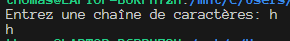
\includegraphics[width=0.8\textwidth]{imgs/execLEC.png}
  \caption{Résultat du l'éxécution du programme avec lecture de données.}
\end{figure}

On voit bien que le programme nous a demandé dans un premier temps d'entrer une chaîne de caractères, puis il nous l'a affichée suite à notre entrée "h". Pour enfin terminer le programme.

\chapter{Conclusion}
Bien que connaître l'Assembleur ne soit pas nécessaire pour la plupart des développeurs, il est important de comprendre les concepts de bas niveau pour apprécier pleinement le fonctionnement des ordinateurs. L'Assembleur est un langage puissant qui offre un contrôle précis sur le matériel, ce qui peut être utile dans des domaines spécifiques comme les systèmes embarqués, les pilotes de périphériques et l'optimisation de code. En apprenant l'Assembleur, on acquiert une compréhension plus profonde du fonctionnement interne des ordinateurs, ce qui peut être bénéfique pour le débogage et l'optimisation des programmes en langages de haut niveau.

\printbibliography

\end{document}